\documentclass[a4paper,12pt]{report}
\setcounter{secnumdepth}{3} % default value for 'report' class is "2"
\usepackage{fullpage}
\usepackage{breakcites}
\usepackage{todonotes}
\usepackage{graphicx}
\usepackage{natbib}
\usepackage{fixltx2e}
\usepackage{titling}
\usepackage{enumerate}
\usepackage{ftnxtra}
\usepackage{mathtools}
\usepackage{textcomp}
\graphicspath{ {images/} }
\usepackage{url}
\usepackage{amsmath}

\widowpenalty 10000
\clubpenalty 10000

\begin{document}
\nocite{*}

\begin{titlepage}
\begin{center}
\Huge
\textbf{Using procedural methods to generate realistic virtual rural worlds}

\includegraphics[width = 400px]{uct_logo.jpg} \\
\large
\vfill
\emph{Minor Dissertation presented in partial fulfilment of the requirements for the degree of Master of Science in Computer Science} \\
\normalsize
\vfill
by \\
\Large
\vfill
\textbf{Harry Long} \\
\normalsize
\vfill
Supervised by: \\
\large
\vfill
James Gain and Marie-Paul Cani \\
\normalsize
\vfill
February 2016
\end{center}
\end{titlepage}

\chapter*{}
\begin{center}
\begin{minipage}{.6\textwidth}
\Large
\emph{I know the meaning of plagiarism and declare that all of the work in this document, save for that which is properly acknowledged, is my own.}
\normalsize
\end{minipage}
\end{center}

\tableofcontents
\listoffigures
\listoftables

%!TEX root = thesis.tex

\chapter{Introduction}
\par
Creating detailed virtual worlds can be a tedious task for artists. Indeed, modelling terrain, vegetation, water streams, rivers, water reserves, soil, rocks, buildings and road networks for large virtual worlds "by hand" can be extremely burdensome. This is especially true when realism is a key requirement. The increase in size and complexity of these virtual worlds mirror that of the processing capabilities of computing hardware. As a consequence, the task is only getting worse.\\

A popular technique to overcome the burden of repetitive tasks is to have them automated. This involves generating algorithms which, given a set of input parameters, generate the required content automatically. This is called \textit{procedural content generation} and has already been successfully applied in different areas of computer graphics including: the generation of non-repetitive textures \cite{Efros1999,Liang2001,Wei2009}, modelling plants \cite{Boudon2012,Fourcaud2008,Guo2011,Lewis1999}, generating terrains \cite{Smelik2009,Gain2009,Doran2010}, generating river networks \cite{Derzapf2011,Emilien} and generating city landscapes \cite{Gain,Kelly2007,Parish2001} (figure \ref{Example of procedurally generated content}) \\
A common difficulty with these methods, however, is finding the appropriate input parameters for the procedural algorithms. The correlation between the parameters and the resulting content is often unintuitive and, as a consequence, often comes down to iterative trial-and-errors until a "close enough" result is found. To overcome this, interactive techniques are often used in an attempt to make generating the input parameters more intuitive. These range from simple paint tools such as lassos and brushes \cite{Emilien} to sketch-based recognition algorithms \cite{Gain2009}. \\

\begin{figure}[h]
  \centering
	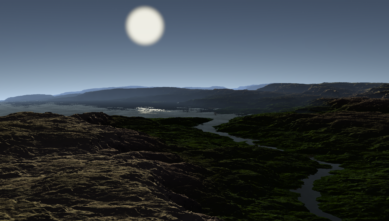
\includegraphics[natwidth=389,natheight=222]{procedural_generated_river.png}
	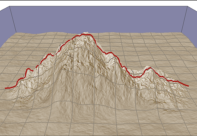
\includegraphics[natwidth=197,natheight=136]{procedural_generated_terrain.png}
	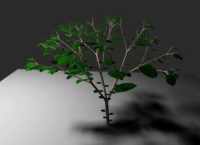
\includegraphics[natwidth=200,natheight=145]{procedural_generated_plant.png}
	\caption{Example of procedurally generated content. From top to bottom, left to right: Procedurally generated river stream \cite{Derzapf2011}, procedurally generated terrain through sketching \cite{Gain2009}, procedurally generated plant \cite{Soler2001}}
	\label{Example of procedurally generated content}
\end{figure}

The intent of this thesis is to develop procedural algorithms to automate the generation of virtual rural worlds. The input parameters for the procedural algorithms must be interactive and/or self-explanatory. 

\newpage
\section{Research Goals}

The research goals for this project are as follows:
\begin{itemize}
\item Develop procedural methods to automate the generation of realistic virtual rural worlds.
\item Provide intuitive and smart controls.
\item When possible, make interactions real-time.
\end{itemize}

One of the most important aspect of rural landscapes is vegetation. As such, our \textit{first goal} must strongly focus on the insertion of plants. The automation provided should not limit user control and the flexibility of the system. For example, it must be possible to generate worlds with varying elevations, river networks, water sources and vegetation.\\

For the \textit{second goal}, lots of thought must be put into making all user oriented controls intuitive. To do so, it will be important to research the pros and cons of other graphical applications in terms of control. If need be, multiple prototype controls should be developed in an attempt to find the best suited.\\

Maintaining a continuous feedback loop between user action and corresponding reaction is extremely important for both user-friendliness and to optimize usage. In an attempt to meet our \textit{third goal} therefore, efficient algorithms must be developed in order to keep there time complexity to a minimum. When suited, these algorithms should be developed to run on the GPU. \\

\section{Contributions}

The primary contributions of this thesis are:
\begin{itemize}
\item A carefully designed graphical interface permitting users to model any environment with minimal effort.
\item An efficient procedural water network generation algorithm which relies solely on soil, rainfall and terrain properties.
\item A novel vegetation generation component which uses clustering, statistical analysis and a simulator to ensure both realism and efficiency.
\end{itemize}

\section{Structure}

To start, a detailed overview of existing work is discussed in chapter \ref{chap:background}. To better understand the individual system components discussed within the body of this text, first an overview of the system is given. This is done in chapter \ref{chap:system_overview}. How the base terrain is specified, associated resources configured and water content procedurally generated is outlined in chapter \ref{chap:terrain_and_resources}. The clustering algorithm used to group vertices based on associated resources is discussed and its performance analysed in chapter \ref{chap:clustering}. Chapter \ref{chap:vegetation} discusses the techniques used to deduce suitable vegetation and efficiently generate highly detailed and large scale plant distributions. Test environments are generated and the systems strengths and weaknesses discussed in chapter \ref{chap:results}. Finally, chapter \ref{chap:conclusion} concludes this thesis and discusses future directions for this work.


%!TEX root = thesis.tex

\chapter{Background}

This chapter gives an overview of previous work related to our topic. Procedural methods applied to computer graphics is a wide area of research with an exhaustive number of publications. As a consequence, we cannot pretend to review all this work. Instead, we will focus on reviewing work which is closely linked to generating virtual \textit{rural} worlds. \\

We first present research which deals with the procedural generation of terrains. This will be followed by a review of methods to generate water flows on terrains. To conclude, an overview of techniques to generate vegetation will be presented.
\section{Rivers and Streams}

In this section will be reviewed the various techniques that are used to place rivers and streams on a terrain. We will split the review material into the following categories, each with dedicated sections: \textit{Classification-based}, \textit{Simulation-based}, \textit{Heuristic-based}, \textit{Fractal-based} and \textit{Explicit}. \textit{Classification-based} methods use pre-classified data based on real-world analysis to determine the most suited water network given a set of user-defined or terrain-defined constraints. \textit{Simulation-based} techniques attempt to simulate natural phenomena such as gravity to determine the water networks on a given terrain. \textit{Heuristic-based} techniques use algorithms based on real-world observation in an attempt to produce a plausible river network on the terrain. \textit{Fractal-based} techniques use recursive algorithms in their attempt to generate plausible river networks. \textit{Explicit} techniques require the user to specify in great detail the path the river should follow on the terrain.\\

The various techniques will be critiqued based on their realism, computational cost, the automation they provide and the amount of control the user has on the resulting scene. 

\subsection{Classification-based}

Classification-based methods use real-world analysis of river networks to determine, based on terrain parameters (slope, soil type, flow intensity, etc.), the types of rivers best suited (stream, cascade, rapid, etc.) to given landscapes.\\

Emilien et al \cite{Emilien2014} use classification-based techniques in their research focused on the lesser explored area of procedurally generated waterfall scenes. They model waterfalls as three separate segments: \textit{running water}, \textit{free-fall} and \textit{pool}. \textit{Running water} segments are parts of the water network in continuous contact with the terrain. \textit{Free-fall} segments are parts which break terrain contact (i.e. waterfall). Lastly, \textit{pool} segments represent the water-basin formed where free-fall segments meet the terrain. \\
Given a terrain, the user models running water and pool segments by defining control points and free-fall segments by defining a parabola. The control points for the running water and pool segments are not constrained to being in contact with the terrain as the terrain will adapt accordingly. The only constraint is that the path must continuously flow downhill. Based on this input, the system calculates plausible water flow intensities which, if required, can be overridden by the user for finer control.\\
The slope and water flow intensity requirements are then used as input to the waterfall classification (figure \ref{fig:waterfall_classification}) in order to determine realistic waterfall scenes to generate.\\

\begin{figure}[h]
  \centering
	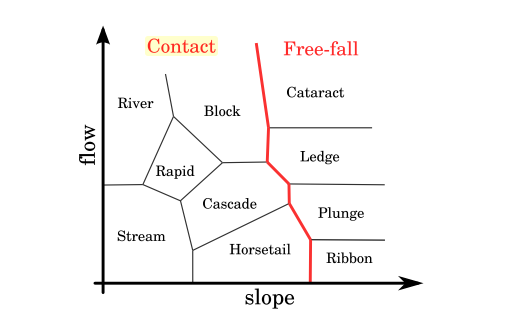
\includegraphics[]{waterfall_classification.png}
	\caption{\textit{Waterfall classifications \cite{Emilien2014}}}
	\label{fig:waterfall_classification}
\end{figure}

By automatically generating plausible waterfall scenes based on trajectory input from the user, the technique strikes a good balance between automation and user control. In terms of computational complexity, the work by Emilien et al \cite{Emilien2014} is able to produce complex waterfall scenes in near real-time.

\subsection{Simulation-based: Gravity} \label{subsec:gravitation}

Gravity simulating techniques attempt to determine the path water will take on a terrain by algorithmically replicating the effects of gravity. \\

In order to generate plausible rivers, Belhadg et Audibert \cite{Belhadj2005} simulate the effect gravity has on water particles placed on the peaks of pre-generated ridges. To create the ridges, particle pairs are first placed at random locations on the terrain. These particle pairs are then randomly assigned a horizontal axis from which they iteratively distance themselves in opposite directions. At each iteration a new vertex is placed and its height decreased from the previous vertex based on a Gaussian distribution. To create the river networks, river particles are placed on the top of these generated ridges and a physical simulation which takes into consideration particle velocity, particle mass and surface friction is used to model the motion of these particles on the terrain. The path followed by these particles is tracked and, when two paths intersect, their particle velocity and mass are combined. When all particles have stopped moving the simulation is deemed balanced and all particle paths which do not lead to terrain extremities discarded. The remaining particle paths are kept and form the core river network. \\

Similarly, in the work by Soon Tee \cite{Teoh2008}, water is placed at specific locations on the terrain either by the user or whilst simulating rainfall. To determine the course the placed water takes on the terrain, water is iteratively evacuated into the surrounding cell with lowest elevation. This continues until a local minima or terrain extremities is reached.\\

In their work on modelling the effects of hydraulic erosion, Št'Ava et al. \cite{StAva2008} determine the course user-placed water takes on the terrain using a hydrostatic pipe-model simulation. In order to do so, the terrain is split into equal-sized (configurable) columns and the simulation iteratively evacuates water from source to surrounding destination columns based on column elevations, fluid density and gravitational acceleration. \\

These techniques can produce very plausible results but have the downside of being dependent on the base terrain as their height-field must cater for river networks in the first place. This is not the case, however, for the work by Št'Ava et al. \cite{StAva2008} for which the gravitation simulation is used as a feedback loop to model terrain erosion. The performance of these methods depend heavily on the level of detail of the underlying water flow simulation. Št'Ava et al. \cite{StAva2008}, for example, succeed in generating the water flow in real-time by optimizing their algorithms to use the heavily parallel architecture of GPUs.

\subsection{Simulation-based: Erosion}

Erosion-based simulations attempt to produce realistic terrains by modelling the effects of erosion. Erosion results from exogenic processes (water flow, wind, temperature) and is characterised by the removal of soil and rock from one location on earth's surface to be redeposited on another. Earth's landscape is a direct consequence of erosion and reproducing this phenomena accurately is core to procedurally generating accurate landscapes. Both Kelly et al. \cite{Kelley1988} and Št'Ava et al. \cite{StAva2008} attempt to produce plausible terrains by modelling these effects.\\

In the work by Kelley et al. \cite{Kelley1988}, the user specifies, on a horizontal plane, the terrain outline along with the main trunk stream. The terrain outline is used to configure the terrain extremities once ported to a three-dimensional space. The main trunk stream specifies the path which the highest order water stream should follow on the resulting terrain. Given this terrain outline and the position of the initial main trunk stream, the system iteratively increments the number of nodes which form the main trunk in order to add streams to the network. The number of new nodes added depends on the drainage area (surface area that a stream needs to channel) and the soil type as more resistant soil materials (e.g. stone) will be less influenced by water erosion than weaker ones (e.g. clay). \\

Št'Ava et al. \cite{StAva2008} are able to simulate the effects of hydraulic erosion on a terrain in real-time by using the massively parallel architectures of GPUs. Virtual pipettes are used by the user to drop water at required locations on the terrain and a gravitation simulation mentioned previously (\ref{subsec:gravitation}) is used to determine the initial water course on the terrain. Whilst the water is being routed through the terrain, the effects of \textit{force-based} and \textit{dissolution-based} erosion are simulated. \textit{Force-based} erosion is a direct consequence of the the force of the water on the terrain surface (figure \ref{fig:force_based_erosion}). Dissolution-based erosion is a consequence of the water mass on the terrain surface under the water and is most often characterised by a smoothing effect (figure \ref{fig:dissolution_based_erosion}).\\

\begin{figure}[h]
  \centering
	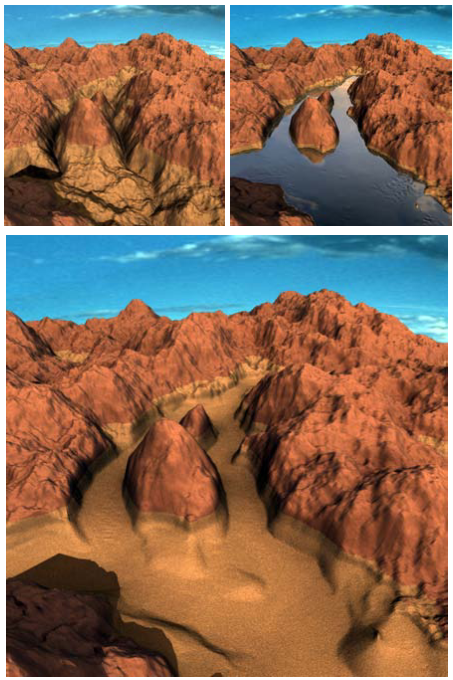
\includegraphics[scale=0.5]{dissolution_based_erosion.png}
	\caption{\textit{Simulation of dissolution-based erosion erosion caused by water movement\cite{StAva2008}}}
	\label{fig:dissolution_based_erosion}
\end{figure}

\begin{figure}[h]
  \centering
	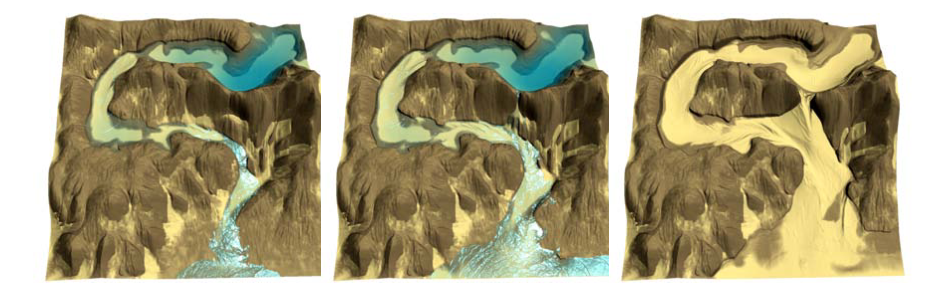
\includegraphics[width=\textwidth]{force_based_erosion.png}
	\caption{\textit{Simulation of the effect of force-based erosion caused by running water \cite{StAva2008}}}
	\label{fig:force_based_erosion}
\end{figure}

Whether modelling erosion indirectly like in the work by Kelley et al. \cite{Kelley1988} which builds the terrain around models of erosion or directly like the work by Št'Ava et al. \cite{StAva2008} which simulates the effect of erosion in real-time, both succeed in producing plausible terrains with integrated river networks. Fine-control over the resulting terrain, however, is limited in the work by Kelley et al. \cite{Kelley1988} due to extensive automation. This is overcome in the work by \cite{StAva2008} et al. by permitting the user to place water using a virtual pipette and remodel the terrain relief on-the-fly. In terms of computational cost, Št'Ava et al. \cite{StAva2008} are able to reproduce the effects of erosion in real-time.  

\subsection{Simulation-based: Rainfall}

In order to determine where on the terrain rivers will appear, work by Soon Tee \cite{Teoh2008} performs a rainfall simulation to determine both the location and quantity of water at different points on the terrain followed by a gravitation simulation (mentioned above) to determine the course of the water on the terrain. The rainfall simulation requires the user to specify wind direction and maximum rainfall. Then, starting from the source of the wind, the system simulates clouds moving in the direction of the wind with a configured velocity. When contact is made with points on the terrain, water is dropped on the corresponding cell. The amount of water dropped increases with altitude and zeroes out when all available rainfall is depleted. \\

Simulating rainfall in order to determine where water will fall on the terrain and therefore where river networks will form is an original approach and one that successfully generates visually plausible terrains. Requiring only wind direction, wind velocity and maximum rainfall from the user, the system provides a good level of automation. Determining the influence these inputs have on the resulting scene could be unintuitive however, and require a "trial-and-error" approach. Their algorithm creates the terrain along with the river networks in O(n) time, n representing the number of cells on the terrain.

\subsection{Heuristic-based}

Heuristic approaches attempt to build river and stream networks on terrains by algorithmically reproducing key characteristics based on real-world observations. \\

Derzapf et al. \cite{Derzapf2011} use such methods in their work based on procedurally generating virtual planets in real-time. To do so, only a very basic mesh-representation of the terrain is generated at first and detailed content is generated on demand as the user navigates through the virtual world. This method of adaptive rendering permits memory usage to me manageable whilst not compromising on realism. To ensure updates are performed in real-time, their algorithms are designed to make use of the massively parallel architecture of GPUs. \\
To initialise the base representation of the planets, the system first creates the base mesh with all vertices representing the sea. The system then randomly assigns a certain number of these vertices to act as seed continent vertices to spread until a user-configured land-to-water ratio is reached.
To place rivers, similarly to the work by \cite{Genevaux2013} et al., they first locate continental points which are on coastal edges to act as river mouths. When such a vertices are found, adjacent continental vertices are iteratively selected pseudo-randomly and connected in order to form the river network. \\
To assign ground altitudes to connected river vertices the system employs the following formula, starting from the river mouth:

\begin{center}
$a_{v} = a_{u} + e_{a}l_{e}\xi , e_{a} = \frac{a_{maxriver}}{l_{r}} $ \\
\end{center}

Where:
\begin{itemize}
\item $a_{v}$ is the ground altitude of the current vertex.
\item $a_{u}$ is the ground altitude of the previously processed vertex (or zero if \textit{v} is the first vertex).
\item $e_{a}$ is the average ground elevation.
\item $l_{e}$ is the length of the current vertex.
\item $\xi \in [0,1[$ is a uniformly distributed pseudo-random number.
\item $a_{maxriver}$ is the user-configured maximum river altitude.
\item $l_{r}$ is the current river length.
\end{itemize}

When the ground altitudes have been assigned, the following formula is used iteratively on each river vertex to assign water altitudes:

\begin{center}
$w_{v} = a_{v} + e_{w}l_{e}, e_{w} = \frac{\epsilon_{river}}{l_{cr}} $
\end{center}

Where:
\begin{itemize}
\item $w_{v}$ is the water altitude of the current vertex.
\item $a_{v}$ is the ground altitude of the current vertex.
\item $e_{w}$ is the average water elevation.
\item $l_{e}$ is the length of the current vertex.
\item $\epsilon_{river}$ is the user-configured maximum river depth.
\item $l_{cr}$ is the distance from the current vertex to the river spring.
\end{itemize}

All randomness in these algorithms depend on a configured seed value enabling the virtual world to be easily reproducible.  \\

This heuristic approach offers an extensive level of automation and, as a result, fine control over the resulting scene is lost. Rather than generating virtual worlds fitting specific user requirements, it is more suited to generating plausible virtual worlds which fit loose constraints (e.g. maximum river altitude, maximum water depth, river stream must flow downhill, etc.). 

\subsection{Fractal-based}

Another technique employed to produce river streams is by employing fractal-based algorithms. Such methods use recursive splitting and string rewriting to determine plausible river networks. 

In their work, Pmsinkiewicz et al. use a fractal-based technique based on midpoint-displacement to procedurally generate plausible rivers on a terrain. Midpoint-displacement is most commonly used for procedurally generating realistic terrain height-maps and works follows follows: Given a starting triangle representing a terrain \textit{A}, midpoint-displacement iteratively subdivides \textit{A} it into four smaller triangles. Each time new triangle vertices are created they are displaced vertically by a random offset. This process is repeated until a given recursion limit is reached. See figure \ref{fig:midpoint_displacement} for an example of a single iteration of the process.

\begin{figure}[h]
  \centering
	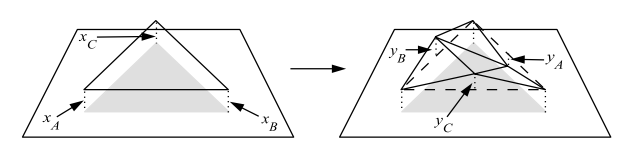
\includegraphics[width=\textwidth]{midpoint_displacement.png}
	\caption{\textit{A single iteration of midpoint displacement for the creation of mountains \cite{Prusinkiewicz1993}. New vertices $y_{A}$, $y_{B}$ and $y_{C}$ are created and shifted vertically by a random offset}}
	\label{fig:midpoint_displacement}
\end{figure}

To adapt this method to the generation of rivers on the terrain, rather than vertically displace newly formed triangle vertices, there edges are labelled as \textit{entry}, \textit{exit} or \textit{neutral} (figure \ref{fig:single_prod_of_midpoint_displacement}). An \textit{entry edge} defines the point of entry for the river into the triangle, an \textit{exit edge} the point of exit and a \textit{neutral edge} prevents the river from passing through. \\

When a production step is applied and a triangle split, the following constraints must be applied:
\begin{itemize}
\item An entry edge must split into an entry and a neutral edge.
\item An exit edge must split into an exit edge and a neutral edge.
\item A neutral edge must split into two neutral edges.
\item The newly formed edge-pairs within the triangle must either be "entry/exit" or "neutral/neutral".
\end{itemize}

\begin{figure}[h]
  \centering
	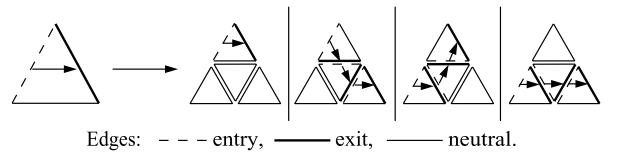
\includegraphics[width=\textwidth]{midpoint_displacement_for_rivers_1.png}
	\caption{\textit{Single production of midpoint displacement adapted to river generation \cite{Prusinkiewicz1993}. Given the initial triangle, four valid split scenarios.}}
	\label{fig:single_prod_of_midpoint_displacement}
\end{figure}

One difficulty with this technique is to ensure two adjacent triangles are coherent once split. That is, that the exit edge of one coincides with the entry edge of the other. To solve this, the location of edge vertices are used as the key to a random number generating hash table which, based on its output number, determines the segment that will be crossed by the river, if any.  \\

In their work, Génevaux et al. \cite{Genevaux2013} use fractal-based string rewriting to produce the river networks on the terrain. Once initial nodes have been selected to act as the river mouth, rewriting grammar is used to perform river node expansion. Configured values of $\rho_{a}, \rho_{s} and \rho_{c}$ influence the probability of selecting productions favouring asymmetric branching, symmetric branching and continuation without branching, respectively. The position for the new node is then selected based on the following constraints:
\begin{itemize}
\item It should be at a minimum distance from existing nodes and edges.
\item The new node should be at a greater distance from the terrain contour.
\item The new node should be compatible with the elevation constraints of existing nodes.
\end{itemize}
If a position satisfying these constraints is found, a new node is added at the given position and the process is repeated.\\

Both these techniques are successful in generating realistic river networks on terrains. The user, however, is limited in the amount of control he has over the resulting rivers. In the work by Génevaux et al. \cite{Genevaux2013}, for example, this is limited to specifying the preferred river branching behaviours. In terms of performance, Génevaux et al. \cite{Genevaux2013} are able to produce terrains of several hundred square kilometres in a matter of seconds.

\subsection{Explicit}

Explicit techniques use explicit input from the user to determine locations and properties of the river networks to generate.\\

Flood-filling is such a technique and is used in the work by Soon Tee \cite{Teoh2008} to permit users to place water reserves (e.g. sea, lakes, etc.) by clicking a single point on the terrain. This point which will act as the seed point for the water surface and will propagate iteratively to surrounding points at lower heights until all such points have been depleted. \\

Smelik et al. also use explicit techniques to create an interactive system permitting users to model a complete virtual world with content ranging from rural features (mountains, rivers, etc.) to man-made ones (buildings, road networks). When modelling the virtual world, interactions are split into two modes: \textbf{Landscape} and \textbf{Feature}. \textit{Landscape mode} permits the designer to paint ecotopes onto the terrain using traditional image editing tools. These ecotopes are predefined by the user and encompass both elevation and soil material information. In \textit{feature mode}, the user is able to place terrain content, including rivers. To do so, similarly to the interface provided by Emilien et al. \cite{Emilien2014}, the user sketches vector lines outlining the core path of the river and, based on this, a suitable course is plotted through the landscape. Other terrain features to which the river takes precedence adapt accordingly. For example, if the river is plotted to pass through a forest, trees on the rived bed and bank will be removed automatically. \\

Rather than placing vector-lines, the work by Soon Tee \cite{Teoh2008} and Št'Ava et al. \cite{StAva2008} permits users to click single points on the terrain which will act as the water source. The system then automatically generates a plausible path for the water down slope of the terrain.\\

As these methods provide very little automation in terms of guaranteeing consistency in the scene, the resulting realism is very much user-dependent. Real-time action-reaction feedback is essential with explicit modelling and so the majority of the methods run in real-time.

\subsection{Summary} \label{Summary}

Each technique has it's associated pros and cons and so choosing which one is best suited depends heavily on the requirements of the system. For example, if the terrain is fixed, using techniques which simulate real-time erosion of the terrain would be ill-suited. Similarly, if fine control over the resulting scene is necessary, heavily automated procedural methods which generate realistic scenes using very little user input would certainly not meet the requirements of the system. In this section we will summarize the pros and cons of the individual techniques in table form. These techniques will be rated based on:
\begin{itemize}
\item \textit{Automation}: The level of automation the technique provides.
\item \textit{Realism}: The realism of generated scenes.
\item \textit{Computational efficiency}: The techniques efficiency in terms of computational resources.
\item \textit{User-control}: How much control the user has over the final scene. 
\end{itemize}

\begin{table}[h]
  \centering
	    \begin{tabular}{|p{4cm}|p{3cm}|p{3cm}|p{3cm}|p{3cm}|}
  	    \hline	
  	      & \textbf{Automation} & \textbf{Realism} & \textbf{Computational Efficiency} & \textbf{User-control} \\
		\hline	
		\textbf{Classification-based} & 
		 %Automation  %Realism  %Comp. Effic. %User-control
		 Good  & Very Good  & Good & Very Good  \\
  	    \hline	
		\textbf{Fractal-based} & 
		 %Automation  %Realism  %Comp. Effic. % User-control
		 Excellent & Good & Good & Poor  \\
  	    \hline
		\textbf{Explicit} & 
		 %Automation  %Realism  %Comp. Effic. %User-control
		 Poor & Fair & Very Good & Excellent   \\
  	    \hline
  	    \multicolumn{5}{|c|}{\textbf{Simulation-based}} \\
  	    \hline				
  	    \textbf{Gravity} & 
		 %Automation  %Realism  %Comp. Effic. %User-control
		 Very Good & Good & Fair & Fair   \\
  	    \hline
		\textbf{Erosion} & 
		 %Automation  %Realism  %Comp. Effic. %User-control
		 Very Good & Very Good & Good & Fair      \\
  	    \hline
  	    	\textbf{Rainfall} & 
		 %Automation  %Realism  %Comp. Effic. %User-control
		 Very Good & Good & Good & Poor      \\
  	    \hline		
  	    \end{tabular}
  \caption{\textit{Summary of river placement techniques}}
	\label{Pros and cons of individual techniques}
\end{table}

In our system, the base terrain will take the form of a preloaded height map. Modifications to this terrain and modelling new terrains will be out-of-scope and, as such, all techniques which require such behaviour can be discarded.\\
Rainfall is a vital requirement to plant life and, as such, gathering rainfall data will be essential to model realistic vegetation on the terrain. Using this rainfall data along with soil properties, it is possible to calculate the amount of standing water which has not been absorbed by the soil. Using this, along with a gravitation simulation, it should be possible to determine main river networks on the terrain based on water builds up. The water drainage simulation employed here will be gravitational based and inspired from the hydrostatic pipe-model of Št'Ava et al. \cite{StAva2008}. It should be optimized to work in real-time and its duration controllable by the user in order to have fine-control over the size and depth of the resulting river networks (i.e. a longer simulation will drain more water and, as such, the river networks will be less intense).

\section{Vegetation}

Vegetation is core to rural landscapes. The species present along with their associated densities create a relationship between ecosystems and areas on earth on which resources are adequate. To ensure realism in virtual environments, much emphasize must be put on efficiently modelling these underlying ecosystems.\\

This section will review different methods to generate suitable vegetation for virtual worlds. These methods can be split into three main categories: \textit{Explicit Instancing, Probabilistic Instancing} and \textit{Plant Growth Modelling}.\\
\textit{Explicit Placement} require explicit user-input to directly or indirectly pinpoint exact locations for individual plant instances.\\
\textit{Probabilistic Placement} methods use statistical models to generate suitable vegetation.\\ 
\textit{Simulators} attempt to algorithmically reproduce plants battling for available resources.\\

We will measure the success of these techniques based on the level of automation they provide, the realism they achieve, their computational cost and their adaptability. Adaptability, here, represents the ease at which a given technique is able to model a number of different vegetation scenarios. \\

\subsection{Explicit Placement} \label{Explicit Placement}
Explicit placement methods require input from the user to determine the location and properties of individual plants. \\

Arnaud et al. \cite{Emilien} permit users to insert individual plants manually by simply clicking a given location on the terrain. To overcome the tedious task of manually placing individual plants on large terrains, the system is able to analyse existing distributions for reproduction. For example, to generate a large forest, the user is only required to generate a small subsection which can then be used to reproduce it on any scale (figure \ref{fig:explicit_placement_input_examplars}) \\

\begin{figure}[h]
  \centering
	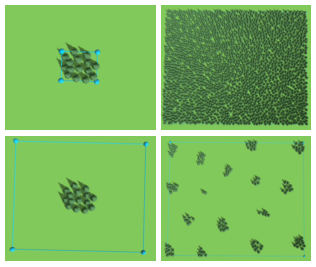
\includegraphics[natwidth=316,natheight=267]{worldbrush_forrest_reproduction.png}
	\caption{\textit{Using explicit placement as input examplars for reproduction \cite{Emilien}}}
	\label{fig:explicit_placement_input_examplars}
\end{figure}

Similarly, Deussen et al. \cite{Deussen1998} allow users to use grayscale raster images as input to specify terrain vegetation. The location of individual plants is determined by pixel location whereas plant properties are correlated to pixel intensity.\\

In their work focused on improving the realism of roadside landscapes, Andujar et al. ~\cite{Andujar2014} use orthophotos as input to determine the location and properties of individual plants. Unlike ordinary aerial photographs, aerial orthophotos use normalisation techniques to take into account terrain relief and camera tilt. The result is an image with uniform scale throughout which, similarly to a map, can be used to accurately measure distances between points. These orthophotos are used to measure the distances between plants. To later reproduce the roadside landscape, they use a dart throwing algorithm to place individual plants whilst respecting the measured distances. \\

\begin{figure}[!htb]
  \centering
	\label{Reconstructed roadside vegetation using orthophotos}
	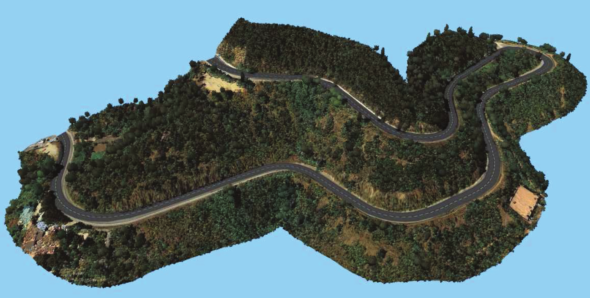
\includegraphics[width=\textwidth]{reconstructed_roadside_vegetation.png}
	\caption{\textit{Reconstructed roadside vegetation using orthophotos ~\cite{Andujar2014}}}
\end{figure}

Explicit placement methods provide significant user control over the resulting virtual world. However, as there is \textit{little to no automation} of this process, it can be very tedious and time consuming for the user. This is especially true when the virtual world being created are very large (e.g. open world video games). An advantage of this limited automation, however, is that modifications are most often very small and are therefore performed in real-time. \\
The \textit{adaptability} of these methods are very poor. Running a different scenario would most often involve starting the entire plant placement process again. \\
Creating vegetation for large virtual worlds using these methods is extremely strenuous and, as a consequence, realism is often compromised.

\subsection{Probabilistic Placement: Radial Distribution Analysis} \label{subsec:prob_placement_radial_dist}

Work by Emilien et al. \cite{Emilien}, Boudon et al. \cite{Boudon2007} and Lane et al. \cite{Lane2002} use radial distribution analysis to convert to metric form the underlying plant distributions of input examplars. The data generated by the analysis stage can later be used to synthesise, at any scale, new point distributions which respect the characteristics of the input exemplar. \\
For example, by analysing the positions of individual plants in a small subset of a forest and using it as the input exemplar, it is possible to reproduce it at a much larger scale in order to model its full size counterpart.\\

\paragraph{Analysis}

Generating the analytical data involves measuring the distances between individual points of different categories from the input examplar. For plant distribution analysis, the points represent individual plants and the categories represent the different species.\\

Before performing the analysis, the following parameters are configured:
\begin{itemize}
\item \textbf{R\textsubscript{min}}: The minimum distance from which point distances need to be analysed.\\
\item \textbf{R\textsubscript{max}}: The maximum distance after which point distances don't need to be analysed.\\
\item \textbf{Bin size}: When analysing the distances of given points, it is necessary to aggregate the points which reside at similar distances into bins. The bin size is the range represented by a single bin.\\
\end{itemize}

A core part of radial distribution analysis is generating pair correlation histograms for each category pair combination. A pair correlation histogram \textit{H\textsubscript{AB}} represents the variation in the distance between points of of category \textit{C\textsubscript{A}} and \textit{C\textsubscript{B}} ranging from \textit{R\textsubscript{min}} to \textit{R\textsubscript{max}} in \textit{bin size} increments (figure \ref{fig:pair_correlation_histograms}) \\

\begin{figure}[h]
  \centering
	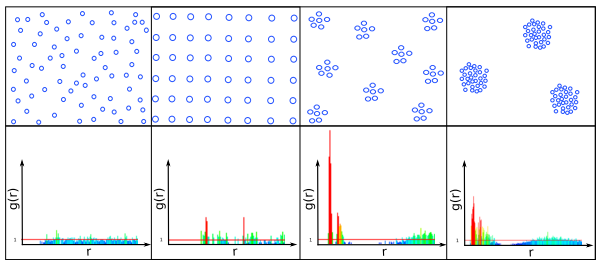
\includegraphics[width=\textwidth]{pair_correlation_histograms.png}
	\caption{\textit{Point distributions with associated pair correlation histogram \cite{Emilien2014}}}
	\label{fig:pair_correlation_histograms}
\end{figure}

To generate the pair correlation histogram \textit{H\textsubscript{AB}}, the algorithm iterates through each reference point of category \textit{C\textsubscript{A}} and, for each destination point of category \textit{C\textsubscript{B}} at a distance between \textit{R\textsubscript{min}} and \textit{R\textsubscript{max}}, increments the relevant bin in the histogram. In figure \ref{fig:radial_distribution_analysis_example}, for example, are being measured the points that lie within the annular shell of radius \textit{r} with bin size \textit{d\textsubscript{r}} (area \textit{d\textsubscript{A}}). 

\begin{figure}[h]
  \centering
	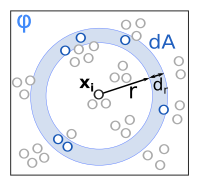
\includegraphics[natwidth=199,natheight=140]{radial_distribution_analysis.png}
	\caption{\textit{Radial distribution analysis}}
	\label{fig:radial_distribution_analysis_example}
\end{figure}

Because of their larger circumference, the coverage area of annular shells get larger as the distance bin being measured increases. In other words, \textit{A\textsubscript{r}} \textless \textit{A\textsubscript{r+1}} where \textit{A\textsubscript{r}} is the area covered by the annular shell starting at distance \textit{r}. A direct consequence of this is that annular shells at further distances will naturally be prone to containing more points. To counter for this, normalisation is performed based on annular shell area. \\

The radial distribution analysis function \textit{h\textsubscript{rdf}} is as follows:\\
\begin{center}	
$h_{rdf}(k) = \sum_{x_{i} \in X} \sum_{y_{j} \in Y \&  
kd_{r} \leq d(x_{i}, y_{j}) < (k+1)d_{r} } \frac{A}{d_{A}n_{x}n_{y}} $
\end{center}
Where:
\begin{itemize}
\item \textit{hrdf(k)} is the k-th value of the pair wise histogram.
\item \textit{X} are the points of category X (reference points).
\item \textit{Y} are the points of category Y (target points)    .
\item \textit{d\textsubscript{r}} is the annular shell width.
\item \textit{A} is the total analysed area.
\item \textit{n\textsubscript{x}} and \textit{n\textsubscript{y}} are the number of points of categories \textit{x} and \textit{y} respectively. Note that pairwise histograms also need to be calculated for points of the same category. In this situation, category \textit{x} and category \textit{y} would be the same.
\item \textit{d\textsubscript{A}} is the area of the annular shell being analysed.
\end{itemize}

Conceptually, this formula calculates the variance from the average density of the target category at incremental distances from points of the reference category.\\

\paragraph{Reproduction}

In order to reproduce the distribution of the input exemplar, points are added iteratively whilst matching as closely as possible the corresponding pair correlation histogram data calculated during the analysis stage. Metropolis-Hastings sampling ~\cite{Hurtut2009} is the most common way to do this. It involves performing a fixed number of point birth-and-death perturbations. A change from the initial arrangement \textit{X} to the new arrangement \textit{X'} is accepted with probability \textit{R}, where:

\begin{center}
$ R = \frac{f(X')}{f(X}$
\end{center}
\textit{f(X)} is the probability density function (PDF) of a given arrangement and is expressed as:\\

\begin{center}
$ f(X) = \prod_{C_{Y_{K}} \leq C_{X}} 
		 \prod_{x_{i} \in X}
		 \prod_{y_{i} \in Y_{k}} 
		 h_{X,Y_{k}}(d(x_{i},y_{j}))$
\end{center} 

Where:
\begin{itemize}
\item \textit{C\textsubscript{y}} and \textit{C\textsubscript{x}} represent categories \textit{Y} and \textit{X}, respectively.
\item \textit{X} are all points of category \textit{X}.
\item \textit{Y} are all points of category \textit{Y}.
\item h\textsubscript{X,Y\textsubscript{k}}(d(x\textsubscript{i}, y\textsubscript{j})) is the value retrieved from the pairwise histogram of categories \textit{X} and \textit{Y} given the distance between points \textit{x\textsubscript{i}} and \textit{y\textsubscript{i}}.
\end{itemize}
Intuitively, the PDF defines, given a set of points, the aggregate strength of the current distribution.\\

Because the PDF formula is a product, calculating it for a new layout \textit{X'} with appended/removed point \textit{P} only involves calculating the PDF for the single reference point \textit{P}. As a consequence, reproduction can be performed very efficiently. In their work, Emilien and Cani ~\cite{Emilien} are able to perform analysis and reproduction in near real-time.\\

When using this technique to reproduce a plausible plant distribution, Boudon et al. \cite{Boudon2007} take it one step further by enabling plant crowns to deform based on predefined elasticity parameters. Because the crowns are not constrained to being circular, they can deform to facilitate the survival of plants at a lower height.

\subsection{Probabilistic Placement: Predefined Ecosystems}

In their work, Hammes el al. \cite{Hammes2001} predefine ecosystems along with their preferred environment. These environments are defined in terms of:

\begin{itemize}
\item Elevation: All plant species have an upper limit after which temperature or oxygen levels are ill-suited.
\item Relative elevation: The local changes in height. Local minimums tend to be valleys and therefore wetter with less illumination. Local maximums, on the other hand, tend to me ridges which are dryer and much more exposed.
\item Slope: Gradient has a direct impact on the quality of the soil and therefore the plants which can grow. When slopes get steeper, plants tend to get much smaller as they struggle to get required nutrients from the soil.
\item Slope direction: This has a direct effect on sunlight exposure. Southern facing slopes in the northern hemisphere will have a greater exposure to the sun and vice-versa for the southern hemisphere.  
\end{itemize}

All these ecosystems are stored in a database and, when vegetation is to be placed on the terrain, the most suitable ecosystems are chosen based on the terrain properties mentioned above. See figure \ref{fig:vegetation_generated_using_predefined_ecosystems} for an example landscape generated using this technique.

\begin{figure}[h]
  \centering
	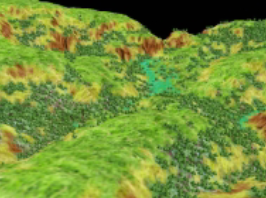
\includegraphics{predefined_ecosystems.png}
	\caption{\textit{Vegetation generated using predefined ecosystems \cite{Hammes2001}}}
	\label{fig:vegetation_generated_using_predefined_ecosystems}
\end{figure}

\subsection{Probabilistic Placement: Conclusions}

\textit{Probabilistic Placement} permit users to specify only small portions of input data to populate large areas. For the \textit{Radial Distribution Analysis} approach, this input data would be in the form of an input distribution. For the \textit{Predefined Ecosystems} approach, it would be a predefined ecosystem along with its preferred environment. Although this automation does ease the task for artists, specifying accurate input data is still crucial to produce realistic vegetation. Consequently, although the realism achieved by these methods is generally good, their adaptability is still limited. \\
Thanks to the use of efficient algorithms, the computational complexity of these methods are often low and real-time updating is achievable. 

\subsection{Simulators: Plant Growth Modelling} \label{subsec:simulators_plant_growth_modelers}

Plant growth modeller attempt to algorithmically reproduce the laws of nature with such precision that they can be used in agronomical sciences and forestry to estimate and maximize crop yield. To achieve this, such simulators go into great detail to model the available resources. For example,  work by Soler et al. ~\cite{Soler2001,Soler2003} splits single plants into geometrical organs with unique light transmittance and reflectance properties. By doing so, light propagation within the plant can be simulated in order to determine the aggregated photosynthetic potential. This work, along with that of Yan et al. ~\cite{Yan2004}, base their simulators on two vital and widely accepted laws of nature:
\begin{itemize}
\item \textit{Law of the sum of temperatures}: Plants grow in cycles which vary from days to years depending on the specie. The law of the sum of temperatures states that the frequency of these cycles is proportional to the sum of the daily average of the temperatures.
\item \textit{Law of the water use efficiency}: The amount of fresh matter fabricated by a plant is proportional to the water evaporation of the plant. This factor is called the water use efficiency. 
\end{itemize}

Water evaporates during photosynthesis as the plant exchanges water for carbon dioxide. Based on this and the law of water use efficiency outlined above, the amount of fresh matter produced (i.e growth) for a given plant is directly correlated to the amount of photosynthesis performed. Using this, Soler et al. ~\cite{Soler2001} apply the following formula to calculate the amount of fresh matter, \textit{Q\textsubscript{m}(t)}, created by a given plant at time \textit{t}:\\

\begin{center}	
\textit{$Q_{m}(t)$} = $\sum_{x=1}^{N(t)} \frac{E(x,t)}{R} $
\end{center}
Where:
\begin{itemize}
\item \textit{E(x,t)} is the potential for matter production of the \textit{x}-th leaf at the \textit{t}-th cycle. It is proportional to the incoming radiant energy up to a certain threshold, after which it remains constant. 
\item \textit{R} is the hydraulic resistance of the given leaf. This resistance is what limits water evaporation (photosynthesis) and therefore growth. It varies depending in the species and surface area.
\end{itemize} 
Intuitively, this formula calculates the total available fresh matter, \textit{$Q_{m}$}, that can be produced for an individual plant \textit{P} at a given time \textit{t}, by calculating the photosynthesis potential of each individual leaf of \textit{P} given the current lighting.\\

Using this, the algorithm iterates through growth cycles with a frequency that is calculated based on the \textit{law of the sum of temperatures} mentioned above. Each growth cycle performs the following two steps:
\begin{enumerate}
\item The lighting and therefore photosynthesis potential of each individual leaf of the plant is calculated. This is then used to calculate, as above, the quantity of fresh matter produced.
\item The fresh matter is then distributed to different organs of the plant according to an associated organ strength.
\end{enumerate}

By going into such detail, these simulators produce very realistic simulations of the evolution of plants. For example, to maximize growth, plants are able to grow in direction of the light source (figure \ref{fig:plant_growing_towards_light_source}).\\

\begin{figure}[h]
  \centering
	    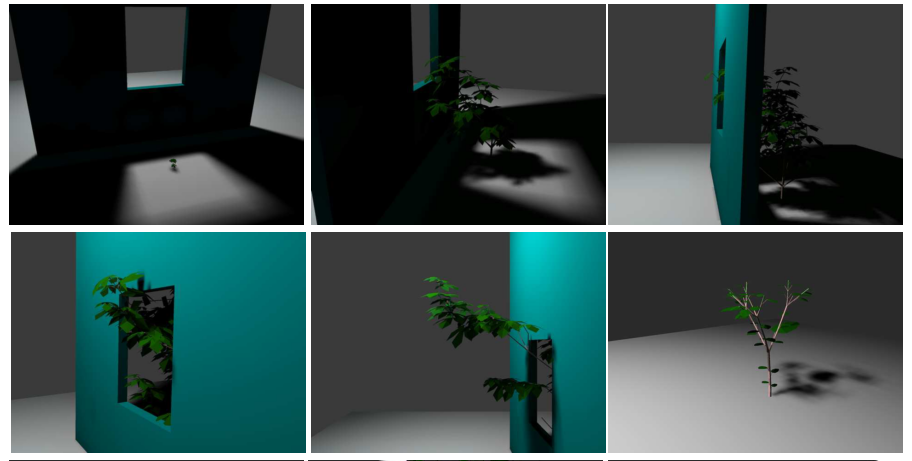
\includegraphics[width=\textwidth]{plant_growing_towards_light_source.png}
	\caption{\textit{Plant growing towards light source ~\cite{Soler2001}}}
	\label{fig:plant_growing_towards_light_source}
\end{figure}

\subsection{Simulators: Ecosystem Simulators} 

Ecosystem simulators use procedural methods to algorithmically reproduce the competition for resources that occurs in nature during plant growth. In nature, this competition is an extremely complex process and so reproducing it exactly would be infeasible. Instead, a simplified model of this ecological process is implemented. During these simulations, available resources fluctuate and each plants strength is continuously recalculated based on its associated properties. This strength directly affects the plants growth and chance of survival. \\
Such plant properties include: age; vigor; shade tolerance; humidity requirement and temperature requirements. Amongst others, the resources modelled include: available illumination; available humidity; temperature and slope.

The aim of ecosystem simulators is to determine, given an initial state \textbf{\textit{S\textsubscript{t}}} of the system at time \textbf{\textit{t}} and a simulation time \textbf{\textit{n}}, the state \textbf{\textit{S\textsubscript{t+n}}}. \\
The state of the system represents individual plant instances with associated location and properties. \\

Lindenmayer systems, commonly referred to as L-systems, use a formal grammar along with a set of production rules to iteratively create larger strings from a starting string called the axiom. Such systems are commonly used to model plants and plant growth ~\cite{Prusinkiewicz1990,Deussen2002,Boudon2012,Prusinkiewicz1993}. \\
An extension to basic L-systems, referred to as open L-systems, adds a communication grammar which permits the set of production rules to behave differently depending on predefined conditions ~\cite{Prusinkiewicz1996}. In their work modelling the growth of struce trees, Berezovskava et al. \cite{Berezovskava1997} use different production rules depending on local bud density. This is a simplified representation of buds competing for available light. \\

By introduction multiset L-Systems, Lane and Przemyslaw ~\cite{Lane2002} extend L-systems yet further to model an ecosystem simulator. The production rules for multiset L-systems work in two stages. The first, identical to basic L-Systems, produces a new string given an input string and production rule. The second, splits the resulting string into new sets using a predefined separation symbol. In their work, the different sets represent different plant instances, thus enabling new plants to spawn during the production steps. When building their L-System, Lane and Przemyslaw ~\cite{Lane2002} focus on reproducing three important properties of nature, each distinctly testable to determine the plausibility of the results:
\begin{itemize}
\item \textit{Self-thinning}: When plants grow, their resource requirements increase and, as a direct consequence, inter-plant competition for resources increases. Eventually, the competition becomes too intense and resources too scarce leading to more vigorous plants starving smaller plants. At this point, self thinning begins and plant densities decrease.
\item \textit{Succession}: Given plant species \textit{A} with a fast growth rate and species \textit{B} with a slower growth rate but higher shade tolerance. At first, the faster growing species \textit{A} will dominate and flourish but, with time, the slower growing but more shade tolerant species \textit{B} will flourish and dominate.
\item \textit{Propagation}: Plants often propagate in clusters surrounding the seeding plant.
\end{itemize}

The L-System they implemented contains different production rules to represent the different properties of nature mentioned above. A single simulation and the corresponding output can be seen in figure ~\ref{fig:plant_placement_using_an_ecosystem_simulator_modelled_by_L_system}.

\begin{figure}[h]
  \centering
    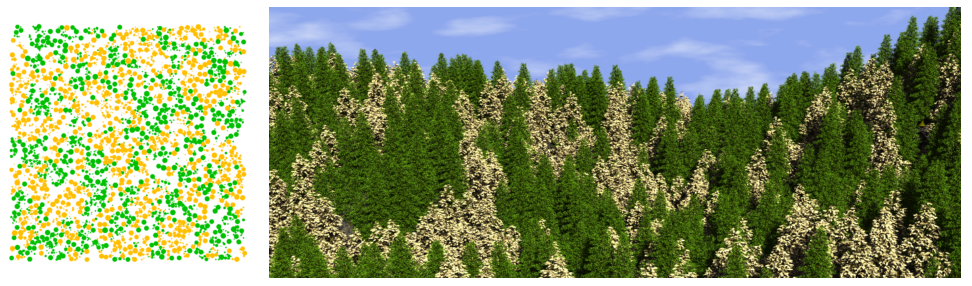
\includegraphics[width=\textwidth]{L-System-Result.png}
    \caption{ \textit{Plant placement using an ecosystem simulator modelled by L-Systems ~\cite{Lane2002}. \textit{Left:} Result of the simulation where orange circles indicate the positions of poplar trees and green circles the positions of spruce trees. \textit{Right:} Reproduced virtual world where the location of individual plants is deduced from the output of the simulator.}}
    \label{fig:plant_placement_using_an_ecosystem_simulator_modelled_by_L_system}
\end{figure}

Work by Deussen et al. ~\cite{Deussen1998} also uses L-Systems as the basis for an ecosystem simulator. As an extension to the work by Lane and Przemyslaw ~\cite{Lane2002}, they introduce the notion of soil humidity and an associated soil per species humidity preference.

A direct consequence of the automation provided by these ecosystems is that fine control over the final vegetation content is lost. Deussen et al. ~\cite{Deussen1998} overcome this, however, by offering a hybrid approach where the ecosystem simulator is first used to populate the entire terrain and explicit instancing is used thereafter for the detailing .\\

Another weakness of procedural ecosystems based on L-Systems worth mentioning is that the communication parameter is binary; in the work by Lane et al. ~\cite{Lane2002} a plant will be dominated as soon as it’s radius intersects another larger plant, at which point it will die with a set probability. This probability of death will stay constant and will not increase as this domination increases. Similarly, in the humidity model of Deussen et al. ~\cite{Deussen1998}, a plant has a preference for wet or dry areas and there is no notion of a measurable humidity preference range. This could prove problematic to model species which are able to adapt to a multitude of environments with varying resource availability (e.g. grass). \\

\subsection{Simulators: Conclusions}
Probably the main advantage of simulators over other approaches is the level of \textit{automation}. Running simulations is done with easy and requires very little input from the user. \\
Although the adaptability of these methods is also impressive, it is limited by the necessity to configure the properties for individual species. This is especially true for \textit{Plant Growth Modelling} approaches where topological data must be configured. Obtaining topological data often involves real-world analysis of the plants growth cycles. \\
Computational cost is often high when using simulators. The extent of which is dependant on the level of detail and the number of plants being simulated simultaneously. For example, in the highly detailed simulations of Soler et al. ~\cite{Soler2001}, simulating 45 cycles for a single plant takes approximately 15 minutes.\\

\subsection{Summary} \label{subsec:vegetation_summary}

Which technique (Explicit, Probabilistic or Simulators) to use entirely depends on the requirements of the system. For example, if realism is the key priority then ecosystem simulators able to provide botanical realism would be the most suitable approach. Choosing the technique is therefore all about minimizing the associated compromises. In table \ref{tab:pros_and_cons_of_vegetation_placement_techniques} we summarize the pros and cons of the individual techniques based on the following criteria: 
\begin{itemize}
\item \textit{Automation}: The level of automation the technique provides. That is, how little user input is needed.
\item \textit{Realism}: The level of realism with which the technique models real-world ecosystems.
\item \textit{Computational efficiency}: The techniques efficiency in terms of computational resource requirements.
\item \textit{Adaptability}: How well the technique can adapt to model different scenarios.
\end{itemize}

\begin{table}[h]
  \centering
	    \begin{tabular}{|p{4cm}|p{3cm}|p{3cm}|p{3cm}|p{3cm}|}
  	    \hline	
  	      & \textbf{Automation} & \textbf{Realism} & \textbf{Computational Efficiency} & \textbf{Adaptability} \\
		\hline	
		\textbf{Explicit Placement} & 
		 %Automation  %Realism  %Comp. Effic. %Adaptability
		 Poor  & Poor  & Excellent & Poor      \\
  	    \hline	
  	    \multicolumn{5}{|c|}{\textbf{Probabilistic Placement}} \\
  	    \hline				
  	    \textbf{Radial Distribution Analysis} & 
		 %Automation  %Realism  %Comp. Effic. %Adaptability
		 Good & Very Good & Very Good & Fair   \\
  	    \hline
		\textbf{Predefined Ecosystems} & 
		 %Automation  %Realism  %Comp. Effic. %Adaptability
		 Good & Fair & Very Good & Poor      \\
  	    \hline
		\multicolumn{5}{|c|}{\textbf{Simulators}} \\
  	    \hline		
		\textbf{Plant Growth Modelling} & 
		 %Automation  %Realism  %Comp. Effic. % Adaptability
		 Excellent & Excellent & Poor & Fair  \\
  	    \hline
		\textbf{Ecosystem Simulators} & 
		 %Automation  %Realism  %Comp. Effic. %Adaptability
		 Excellent & Very Good & Fair & Good   \\
  	    \hline
  	    \end{tabular}
  \caption{\textit{Summary of vegetation placement techniques}}
  \label{tab:pros_and_cons_of_vegetation_placement_techniques}
\end{table}

Given a set of plant species, available resources and terrain, our system must be able to specify the locations of individual plants. The output must be: visually realistic; easily scalable in order to be able to re-run simulations with different input species; computationally efficient to ensure the effect of user actions appear in close to real-time. \\
Given these requirements, a hybrid approach is best suited which combines the adaptability and realism of ecosystem simulators with the computational efficiency of probabilistic placement. Computationally expensive ecosystem simulator runs will be performed beforehand in order to acquire the necessary distribution data. This data will then be stored in order for it to be queried at a later stage without having to redo expensive simulations. When placing vegetation in the virtual world, pre-calculated distribution data will be queried and probabilistic instancing used to fill user-defined areas with suited plant species and realistic distributions. \\

\chapter{Terrain and Resources} \label{chap:terrain_and_resources}

The first step in creating virtual worlds is specifying the base terrain on which features will be placed. Subsequently, terrain resources with direct influence on content are determined. In order to strike a good balance between resulting realism and user experience, procedural methods must be employed when suited.\\
This chapter discusses how a system fitting these requirements was built. The discussion is split into the following core sections: \textit{Terrain \& Navigation}, \textit{Resources}, \textit{Rivers \& Streams}, \textit{Water Reserves} and \textit{Results}.\\
\textit{Terrain \& Navigation} discusses how the base terrain is selected and navigated through. \\
In order to determine suitable vegetation and river sources, resource data needs to be specified. How this is done is discussed in the \textit{Resources} section.\\
Essential to the realism of virtual terrains is water placement. This water can take the form of rivers and streams or water reserves. Techniques used to place such content are discussed in the \textit{Rivers and Streams} and \textit{Water bodies} sections, respectively. \\


\section{Terrain and Navigation}

In order to give the user the freedom to model any type of virtual world, providing the ability to specify any type of base terrain is essential. Efficiently rendering and navigating this terrain is also key for both the user experience and visual realism. How our system manages these requirements are discussed sections \textit{Loading Terrain}, \textit{Rendering Terrain} and \textit{Navigating Terrain} below.

\subsection{Loading Terrain}

As stated previously, our work focuses on terrain content and not terrain relief modelling. As such, the user is only able to load a static, pre-generated terrain in the form of a Terragen height-map. A height-map is a 2-dimensional grid of height values which, once loaded and converted, represents the height of the terrain on a regular grid. The Terragen file format is a freely available and widely used file-specification created by PlanetSide \protect\footnotemark \footnotetext{\url{http://www.planetside.co.uk}} for their realistic virtual world generation software, Terragen. The format wraps raw height data with other important information essential to accurate rendering such as base height, scales and dimensions.\\
Note that modelling the base terrain as static is a simplification as in reality it is affected by erosion. The extent of which depends on many factors including wind, vegetation and water.

\subsection{Rendering Terrain}

Once parsed, the height-map data is transferred to the GPU as a two dimensional texture for rendering. In order to better visualize the terrain relief, a Blinn–Phong shading model is used when rendering the terrain.
This shading model takes into consideration camera viewpoint and lighting incidence angles to determine the influence of diffuse and specular lighting on individual terrain vertices. This information is subsequently used to calculate a weighted contribution of ambient, specular and diffuse colors to determine the aggregate color of individual terrain vertices. By accurately modelling specular and diffuse highlights, renders are more realistic and shapes more distinguishable \citep{Blinn}. By employing this model in this work, terrain relief is made clear.\\
Essential to the Blinn-Phong shading model are the normal vectors for each terrain vertex. This is done using the algorithm outlined in equation \ref{eq:normals_calculation} and illustrated in figure \ref{fig:normals_calculation}. Each normal is calculated in parallel on the GPU, thus ensuring real-time results.

\begin{equation} \label{eq:normals_calculation}
N_{P} = V_{ac} \times V_{db}
\end{equation}
Where: $N_{P}$ is the normal vector at point P and $P_{A}$, $P_{B}$, $P_{C}$ and $P_{D}$ are the direct points surrounding P in the X and Y direction (see figure \ref{fig:normals_calculation}).

\begin{figure}[h]
\center
	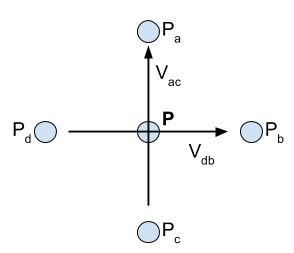
\includegraphics[width=\textwidth/2]{normals_calculation.png}
	\caption{Illustration of the vertices and vectors used to calculate terrain normal at position \textit{P}.}
	\label{fig:normals_calculation}
\end{figure}

\subsection{Navigation}

In order for users to successfully and intuitively navigate through virtual worlds, it is important to prevent disorientation by ensuring continuous user awareness of location and orientation \cite{Darken1993}. 
In their work, Darken et al. \cite{Darken1993} explore various navigation techniques to do so, including the flying scenario where users explore virtual worlds as if they were flying through it. This navigation technique provides a birds eye view of the virtual worlds and enables users to gain an overview of the terrain and efficiently locate landmarks to serve as point of references. Locating such landmarks proves extremely useful in keeping the user aware of his location and therefore preventing disorientation \cite{Darken1993}. Birds eye has become the most widespread navigation technique employed in video games, simulators and virtual world generation software. In order to support a variety of users (novice to computer graphic experts), this is the navigation style used in our system. To further prevent disorientation, a compass is continuously displayed stating the current heading. \\

Intuitive controls and suitable sensitivity thereof are also essential. The correlation between key-press and mouse movement must be predictable so that the user can navigate in three dimensional space without losing his bearings. In an attempt to cater for the control requirements of a wider user-base, two different control types are available in this system: \textit{keyboard-driven} and \textit{click-and-drag}. Details of which can be found in table \ref{tab:control_types}. The active control type is easily configurable, along with sensitivity parameters, through the application's configuration interface.

\begin{table}[h]	
  \centering
	    \begin{tabular}{|p{2.5cm}|p{2.25cm}|p{2.25cm}|p{2.25cm}|p{2.25cm}|p{2.25cm}|}
  	    \hline	
  	    \textbf{Control-type} & \textbf{Translate Left/Right} & \textbf{Translate Up/Down} & \textbf{Translate Front/Back} & \textbf{Rotate Left/Right} & \textbf{Rotate Up/Down} \\
		\hline
		\textbf{First-Person} & A/D key-press & - & W/S key-press & Horizontal mouse movement & Vertical mouse movement \\
		\hline
		\textbf{Click-and-drag} & Horizontal click \& drag & Vertical click \& drag & Scroll wheel & Ctrl + horizontal click \& drag & Ctrl + vertical click \& drag\\
		\hline
		\end{tabular}
		\caption{Control types instruction sheet}
		\label{tab:control_types}
\end{table}


\section{Resources}

\section{Rivers \& Streams}

Essential to the realism of virtual rural terrains are water networks which take the form of rivers and streams. These rivers form as run-off water is being transported by gravity from higher to lower grounds. In this section is  The algorithm used to model gravity and therefore the evacuation of water on any terrain is outlined below along with details on the GPU implementation used to accelerate the process.

\subsection{Water Evacuation Algorithm} 

Precipitation, precipitation intensity and soil infiltration are used to calculate the soil humidity, $S_{h}$, which equates to the quantity of water, in millimetres, absorbed by the soil. The water which isn't absorbed by the soil, \textit{W$_{standing}$} for a given terrain vertex can therefore be deduced using equation \ref{eq:standing_water_calculation}

\begin{equation} \label{eq:standing_water_calculation}
	W_{standing} = R_{q} - S_{h}
\end{equation}
where:
\begin{itemize}
\item \textit{W$_{standing}$} is the standing water, in millimetres.\\
\item \textit{R$_{q}$} is the monthly rainfall quantity, in millimetres.\\
\item \textit{S$_{h}$} is the quantity of water absorbed by the soil, in millimetres.\\
\end{itemize}

Similarly to the work by Stava et al. \cite{StAva2008}, a water evacuation algorithm is used where water is iteratively evacuated from source to destination vertices.

\subsection{GPU Implementation}

through the evacuation of run-off water from higher to lower altitudes and, eventually, 

Water networks form due to the evacuation of 


\bibliographystyle{alpha}
\bibliography{MyCollection}{}
\end{document}